\documentclass[twocolumn]{llncs}

\usepackage{graphicx}
\usepackage{amssymb}
\usepackage{amsmath}
\usepackage[legalpaper, margin=0.8in]{geometry}
\usepackage{soul}
\usepackage{xcolor}

\setlength{\columnsep}{0.3in}

% Constant values
\newcommand{\NCMR}{31,803\,} % Number of individuals
\newcommand{\NCALLS}{801,526\,} % Number of genotyped SNPs 
\newcommand{\MAFTHR}{1\%} % MAF threshold (in percentage)
\newcommand{\NIMP}{10,000,000\,} % number of imputed variants with MAF > threshold
\newcommand{\HWEPVAL}{1e-4} % Hardy-Weinberg equilibrium p-value threshold
\newcommand{\LVNP}{2,677} % number of points in the LV mesh
\newcommand{\LVENDONP}{880} % number of points in the LV
\newcommand{\NGWASHITS}{10}

% ANONYMIZED VERSION 
%\newcommand{\ACCESSIONNUMBER}{---}

\newcommand{\ACCESSIONNUMBER}{11350}

\begin{document}

\titlerunning{Abbreviated paper title}
% If the paper title is too long for the running head, you can set
% an abbreviated paper title here

\twocolumn[
\begin{@twocolumnfalse}
\title{GWAS of CMR-Derived LV Morphology Represented Via Graph-Convolutional Autoencoders in 30k UK Biobank Subjects}

\author{Rodrigo Bonazzola\inst{1,2} \and
Andres Diaz-Pinto\inst{1,2} \and
Rahman Attar\inst{1,2} \and
Nishant Ravikumar\inst{1,2} \and
Eylem Levelt\inst{2} \and
Sven Plein\inst{2}
Enzo Ferrante\inst{3} \and
Tanveer Syeda-Mahmood\inst{4}\and
Alejandro F Frangi\inst{1,2}}

%
% \authorrunning{F. Author et al.}
% First names are abbreviated in the running head.
% If there are more than two authors, 'et al.' is used.
%

\institute{Centre for Computational Imaging and Simulation Technologies in Biomedicine (CISTIB), School of Computing and School of Medicine, University of Leeds, Leeds, UK \and
Leeds Institute of Cardiovascular and Metabolic Medicine, School of Medicine, University of Leeds, Leeds, UK \and
Research Institute for Signals, Systems and Computational Intelligence, sinc(i), FICH-UNL / CONICET, Santa Fe, Argentina \and
IBM Almaden Research Center, San Jose, USA}
\maketitle              % typeset the header of the contribution
\begin{abstract}
The genetic basis of cardiac phenotypes is not yet well understood. Cardiac magnetic resonance (CMR) images, a rich source of structural phenotypes, as well as linked genotype information, were recently made available within the UK Biobank project. Subsequently, a genome-wide association study (GWAS) for left-ventricular (LV) function indices was published using this data, reporting novel genetic loci significantly associated with these phenotypes. However, LV morphological features are yet to be studied in this context. In this work, we performed dimensionality reduction on 3D LV meshes generated from CMR images, which allows us to learn non-local morphological features that constitute a latent basis for the shape. To this end, we used two approaches i) principal component analysis (PCA) and ii) graph-convolutional autoencoders. GWAS was performed on the components of the latent space obtained through each of the methods. Novel genetic loci were discovered which have not been reported in literature, in addition to other loci already known to be associated with cardiac phenotypes. Some of these features were found to be related to cardiac diseases, showing the potential of our approach to pinpoint genetic loci of clinical relevance.
\keywords{Cardiac MR  \and GWAS \and Graph-Convolutional Autoencoders.}
\end{abstract}
  \end{@twocolumnfalse}
]
%

\section{Introduction}

Cardiovascular diseases are the main cause of mortality worldwide.
The recent advances in cardiovascular imaging has allowed for a more accurate phenotyping of the heart, due to the increasing availability of high resolution images from different techniques. Such techniques include echocardiography, nuclear imaging, computerized tomography (CT) and cardiac magnetic resonance (CMR), and are used both in research and in clinical practice.

Some of these image-derived phenotypes (IDPs) are known to have underlying genetic factors, and also to be associated with cardiovascular risk.

The UK Biobank (UKB) is a prospective cohort study that between 2006 and 2010 recruited around half a million volunteers across the United Kingdom, aged 40-69 years old at the time of recruitment \cite{ref_ukbb}. This sample aims to be representative of the whole UK population. The project collected a huge amount of phenotypic information about its participants, and also linked them to their electronic health records (EHR). The collected data include, among others, genetic data from SNP microarrays for all the individuals, and also CMR data for a subset of the participants (which as of the time of this writing is of more than 40,000 individuals but is planned to reach 100,000 by 2023.) These datasets are described in \cite{ref_ukbb_genetics} and \cite{ref_ukbb_cmr}, respectively.

On the other hand, genome-wide association studies (GWAS) have been very successful in identifying genetic variants associated with a broad range of phenotypes \cite{ref_gwas_review}. To the best of our knowledge, only two studies have been published so far in the field of cardiac imaging genetics using CMR data. However, the breadth of cardiovascular IDPs studied in this context has been hitherto limited to those with known clinical relevance. These include the volumes of the different cardiac chambers, parameteres related to the function of the heart (such as stroke volume, cardiac output and ejection fraction of the chambers) and myocardial thickness and mass.

The first one \cite{ref_biffi} studies left-ventricular wall thickness at end-diastole, performing an association test with a set of genetic variants in a vertex-by-vertex fashion.

In the second one \cite{ref_nayaung}, the authors focused on CMR imaging data from nearly 17,000 UK Biobank participants and processed it to obtain 6 left-ventricular IDPs: 1) end-diastolic volume (LVEDV), 2) end-systolic volume (LVESV), 3) stroke volume (LVSV), 4) ejection fraction (LVEF), 5) mass (LVM) and 6) mass-to-EDV ratio (LVMVR).

However, instead of extracting handcrafted features from the images (such as the ones mentioned above), the unprecedented amount of linked genetic and cardiac imaging data available within the UK Biobank allows for a different kind of approach: techniques of unsupervised machine learning can be employed in order to automatically learn a set of features that best describe the morphology of the heart. 
The hypothesis is that these learnt features, by virtue of its greater variability across the population, will be good candidate IDPs on which to perform genetic association analysis, in the sense that some of them would be expected to be largely heritable.

The contributions of this paper are threefold. Firstly, we reproduce the results in \cite{ref_nayaung} using a superset of \NCMR\, UKB participants, and extend the analysis to consider the equivalent quantities for the other three cardiac chambers: right ventricle (RV), left atrium (LA) and right atrium (RA).
Secondly, we prove that a deep-learning-based dimensionality reduction method (namely, an autoencoder with convolutional layers) allows to reconstruct the different chambers with an acceptable error, and that the learnt space has an easy morphofological interpretation. Thirdly, we perform GWAS on the components of this latent space.

\section{Methods}
The workflow is shown in figure \ref{fig:workflow}.

\begin{figure}
\centering
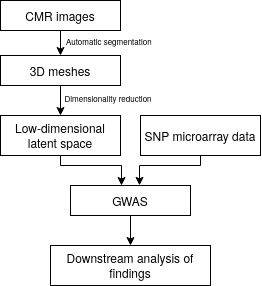
\includegraphics[width=0.8\linewidth]{figs/workflow.png} 
\caption{Flowchart of the steps performed in this work}
\label{fig:workflow}
\end{figure}

\subsection{Description of the data}
The data used for this work comes from the UKB project, data accession number \ACCESSIONNUMBER.

\subsubsection{CMR data and its processing.}
The CMR imaging protocol used to obtain the raw imaging data is described elsewhere \cite{ref_ukbb_cmr}. 

\paragraph{Segmentation algorithm.}
The CMR images were segmented automatically using an algorithm that is described in detail in \cite{ref_rahman}, the output of which is a set of 3D meshes, one per subject and per time point.

Each cardiac mesh, $\mathcal{G}_{i}^{(t)}$, consists of a set of vertices and edges $\mathcal{G}_{i}^{(t)}=\{\mathcal{V}_{i}^{(t)}, A_{i}^{(t)}\}$ describing the shape for individual $i$ at instant $t\in[0,1)$ of the cardiac cycle. The cardiac period is normalized to 1 for each individual and $t=0$ is the end-diastolic phase %(whereas end-systole varies across individuals but lies typically in the range ??? 18-19/50).
\footnote{Notice that in order to convert from these normalized time units to real time units, the pulse rate needs to be used.}. In this work, we only investigate $t=0$ (end-diastole), so the temporal superindex will be dropped in the following. Each element of $\mathcal{V}_i$ is a 3D point $\textbf{x}_{ij}=(x_{ij}, y_{ij}, z_{ij}),\, j=1,...,M,\ i=1,...,N$, and $A_{i}\in\{0,1\}^{M\times M}$ is the adjacency matrix of the mesh, where $(A_i)_{j_1j_2}=1$ if and only if there is an edge between vertices $j_1$ and $j_2$ in the mesh of subject $i$.
\textcolor{red}{Probably I should add an index to denote the cardiac chamber.}


In our particular case, this becomes significantly simpler since the connectivity of the meshes is inherited from a reference atlas, and thus all the meshes have not only the same number of vertices but also the same connectivity, both across individuals and across phases; i.e. $M=|\mathcal{V}_k|=|\mathcal{V}_l|$ and $A:=A_{k}=A_{l}$, $\forall k, l$.

 %An alternative way to express the connectivity of the mesh is through the adjacency matrix , where $A_{ij}=1$ if vertex $i$ is connected to vertex $j$, and is zero otherwise. This way of representing the connectivity is useful in the context of spectral graph theory, as will be explained in more detail in subsection \ref{results:dimensionality_reduction}.

% Each element of $\mathcal{V}_i$ is a 3D point $\textbf{x}_{ij}=(x_{ij}, y_{ij}, z_{ij}),\, j=1,...,M,\ i=1,...,N$, and $(\textbf{x}_{ij_1}, \textbf{x}_{ij_2})\in\mathcal{V}_i$ means that there is an edge between vertices $j_1$ and $j_2$ in the cardiac mesh of subject $i$ at time $t$. In our particular case, this becomes significantly simpler since the connectivity of the meshes is inherited from a reference atlas, and thus all the meshes have not only the same number of vertices but also the same connectivity, both across individuals and across phases; i.e. $M=|\mathcal{V}_k^{(t_1)}|=|\mathcal{V}_l^{(t_2)}|$ and $A:=A_{k}=\mathcal{E}_{l}^{(t_2)}$, $\forall k, l, t_1, t_2$.

%Each cardiac mesh, $\mathcal{G}_{i}^{(t)}$, consists of a set of vertices and edges $\mathcal{G}_{i}^{(t)}=\{\mathcal{V}_{i}^{(t)}, \mathcal{E}_{i}^{(t)}\}$ describing the LV shape for individual $i$ at instant $t\in[0,1)$ of the cardiac cycle, where the cardiac period is normalized to 1 for each individual and $t=0$ is the end-diastolic phase (whereas end-systole varies across individuals but lies typically in the range ??? 18-19/50). Notice that in order to convert from these normalized time units to real time units, the pulse rate needs to be used.

% \footnote{CLARIFICATION (This could go to supplementary material): in more rigor, the endocardial and epicardial meshes are derived each from a different atlas and then a merging procedure is applied in order to obtain a single mesh for both walls. Notice that since the whole shape does not come from one single atlas, there is no guarantee that the connectivity of the resulting mesh will be the same for different individuals (it depends on the nature of the merging procedure selected, and if it is based on distances between vertices, it could certainly not be the case since the neighboring vertices in different meshes). To overcome this inconvenient situation, the merging procedure is applied to a single mesh, and the resulting connectivity is applied to the rest of the meshes.}

% An alternative way to express the connectivity of the mesh is through the adjacency matrix $A\in\{0,1\}^{M\times M}$, where $A_{ij}=1$ if vertex $i$ is connected to vertex $j$, and is zero otherwise. This way of representing the connectivity is useful in the context of spectral graph theory, as will be explained in more detail in subsection \ref{results:dimensionality_reduction}.


\subsubsection{Genotypic data}
SNP microarray data is available for all the individuals in the UK Biobank cohort. This microarray covers \NCALLS\, genetic variants including SNPs and short indels. The design of this microarray has been described in detail in %\cite{ref_ukbb_genetics}
. From these genotyped markers, an augmented set of \NIMP variants was imputed. The GWAS was performed across this latter set, filtering by a minor allele frequency (MAF) threshold of \MAFTHR and a HWE p-value threshold of \HWEPVAL.


\subsection{Dimensionality reduction}
\label{results:dimensionality_reduction}

\paragraph{Mesh pre-processing.} First of all, the pose nuisance parameters (translation, rotation and scaling) are removed using generalized Procrustes analysis. 
Given a set of 3D shapes % $\textbf{s}_i^{(t)}=(x_{i1}^{(t)}, y_{i1}^{(t)}, z_{i1}^{(t)}, ..., x_{iM}^{(t)}, y_{iM}^{(t)}, z_{iM}^{(t)})\in \mathbb{R}^{3M}$,
$\textbf{s}_i=(x_{i1}, y_{i1}, z_{i1}, ..., x_{iM}, y_{iM}, z_{iM})\in \mathbb{R}^{3M}$,
we derive the mean shape and the shape covariance matrix:

\begin{equation}
\bar{\textbf{s}}=\frac{1}{N}\sum_{i=1}^{N}{\textbf{s}}_i,
\end{equation}

\begin{equation}
\textbf{S}=\frac{1}{N-1}\sum_{i=1}^{N}({\textbf{s}}_i-\bar{\textbf{s}})({\textbf{s}}_i-\bar{\textbf{s}})^t.
\end{equation}

In order to extract a reduced set of features that describe left-ventricular shape, two methods were utilised: principal component analysis (PCA) and mesh-convolutional autoencoders. In the first case only 3D point clouds are provided as input, whereas in the second case we also leverage information about connectivity between the vertices. However, both approaches can be thought of as special cases of a common paradigm.

In such paradigm, there is a pair of encoding and decoding functions, $E_{\theta_E}:\mathbb{R}^{3M}\rightarrow\mathbb{R}^{K}$ and $D_{\theta_D}:\mathbb{R}^{K}\rightarrow\mathbb{R}^{3M}$ that are parameterized by a set of parameters $\theta_E$ and $\theta_D$, respectively. $K$ is usually chosen so that $K\ll M$ (hence the dimensionality reduction). 

The optimal parameters $\theta_E^*$ and $\theta_D^*$ for reconstruction can be learnt by making the composite function $D_{\theta_D} \circ E_{\theta_E}$ as close to the identity function $I$ as possible for the data in the training set, using some reasonable loss function such as the squared $L_2$ norm of the element-wise difference, along with a regularization term $\Omega$; that is to say

\begin{equation}
L_2^2(\textbf{s}|\theta_E, \theta_D)=
\sum_{i=1}^{N} \big|\big|\big(D_{\theta_D} \circ E_{\theta_E} - I\big) (\textbf{s}_i) \big|\big|_2^2
\end{equation}

\begin{equation}
L(\textbf{s}|\theta_E, \theta_D)= L_2^2(\textbf{s}|\theta_E, \theta_D) + \lambda\Omega(\textbf{s}|\theta_E, \theta_D)
\end{equation}

\begin{equation}
(\theta_E^*, \theta_D^*) = \text{argmin}_{\theta_E, \theta_D}L(\textbf{s}|\theta_E, \theta_D).    
\end{equation}{}

%\begin{equation}
%(\theta_E^*, \theta_D^*) = \text{argmin}_{\theta_E, \theta_D}\mathrm{E}_{}\bigg( \big|\big|\big(D_{\theta_D} \circ E_{\theta_E} - I\big) (\textbf{s}_i) \big|\big|_2^2.    
%\end{equation}{}

$\textbf{Z}_i:= E_{\theta_E^*}  (\textbf{s}_i)\in\mathbb{R}^{K}$ would then be a low-dimensional representation of the shape $\textbf{s}_i$, whereas $\hat{\textbf{s}}_i:=\big(D_{\theta_D^*} \circ E_{\theta_E^*}\big)(\textbf{s}_i)$ is the associated reconstructed shape.

\subsubsection{Principal component analysis.}
PCA is a standard linear technique for dimensionality reduction. In terms of the framework detailed above, it can be obtained by requiring $D$ and $E$ to be linear transformations/mappings and using the $L_2$ norm.

The idea is to find a basis of vectors $\mathcal{B}_{K}=\{\textbf{v}_i\}_{i=1}^{K}\subset\mathbb{R}^{3M}$ for a fixed $K < 3M$, such that the $K$-dimensional linear subspace generated by $\mathcal{B}$ captures as much of the shape variability as possible. It can be shown that such basis corresponds to the $K$ eigenvectors of the $\textbf{S}$ matrix with the top largest eigenvalues; i.e. if $\textbf{S}=\Omega^{t}\Lambda\Omega$ where $\Lambda=\delta_{ij}\lambda_i$ and $\lambda_i \geq \lambda_j$ if $i\leq j$, then $\mathcal{B}_{K}=\{{\Omega\textbf{e}_i}\}_{i=1}^{K}$.

% One of the drawbacks of this approach is that by the linear nature of the encoding and decoding function, it is unable to capture non-linear features of the shapes.

%In other words, $\mathcal{B}$ represent the $K$ directions in $\mathbb{R}^{3M}$ of greater variability in left-ventricular shape.

\subsubsection{Convolutional mesh-AE.}

In an autoencoder, both the encoding and decoding functions are feed-forward neural networks.
In the particular method employed in this work (published in \cite{ref_coma} and based, in turn, on previous work published in \cite{ref_spectral_graph_conv}), each layer of the encoder and decoder implements convolution operations, in order to leverage information about the local context of each vertex. Furthermore, in order to learn global features, a hierarchical approach is used where each layer of the encoder and decoder implement downsampling and upsampling operations, respectively. 
 
Since the vertices are not in a rectangular grid, the usual convolution, pooling and unpooling operations defined for such geometry (usually employed in image analysis) are not adequate for this task and need to be suitably adapted. There is a number of methods to do this, but they all can be classified into two large groups: spatial or spectral. In this work we'll apply a method belonging to the latter category, which relies on expressing the features in the Fourier basis of the graph, as will be explained below.

The Laplace-Beltrami operator of a graph with adjacency matrix $A$ is defined as
\begin{equation}
\mathcal{L}=D-A,
\end{equation}{}
\noindent 
where $D$ is the degree matrix, i.e. a diagonal matrix where $D_{ii}=\sum_{j}A_{ij}$ is the number of edges that connect to vertex $i$. The Fourier basis of the graph can be obtained by diagonalizing the Laplace operator, $\mathcal{L}=U^t\Lambda U$. The columns of $U$ constitute the Fourier basis, and the operation of convolution $\star$ for a graph can be defined in the following manner

\begin{equation}
x\star y =U(U^tx\odot U^ty)
\end{equation}{}

\noindent where $\odot$ is the element-wise product (also known as Hadamard product)
\footnote{Can $\textbf{S}$ (the covariance matrix) be thought of as the adjacency matrix of a weighted graph and thus the principal components are just the elements of the Fourier basis of this weighted graph?}

All spectral methods for convolution rely on this definition of convolution, and differ from one another in the form of the kernel/filter utilized. In this work, a parameterization proposed in \cite{ref_spectral_graph_conv} will be used. 
Said method is based on the Chebyshev polynomials $\{T_i\}$. The kernel $g_\xi$ is defined as

\begin{equation}
g_{\xi}=\sum_{i=1}^{K}\xi_i T_i.
\label{eq_chebyshev_filter}
\end{equation}

Chebyshev polynomials have the advantage that they can be computed recursively through the relation $T_i(x)=xT_{i-1}(x)-T_{i-2}(x)$ and the base cases $T_1(x)=1$ and $T_2(x)=x$. The filter described by equation \ref{eq_chebyshev_filter} also has the characteristic of being local (EXPAND ON THIS)

The sampling and upsampling operations in this work were proposed in \cite{ref_coma}. In each layer, the sampling operations generate a subgraph of the graph in the previous layer, such that the quadric error is minimized \cite{ref_quadric_error}. The upsampling operations are created while performing the downsampling: the coordinates of the decimated vertices with respect to the remaining vertices are stored for each layer.

In this work, the input to the autoencoder is a modified version of the shapes $\textbf{s}_i\mapsto \textbf{t}_i\equiv(\textbf{s}_i-\bar{\textbf{s}})/\textbf{S}_{ii}$. \textcolor{red}{Actually, the input to the network belongs to $\mathbb{R}^{M\times 3}$, i.e. is a matrix where each channel  (column) corresponds to one spatial coordinate, but I need to come up with a good notation for this. The way it's written now makes it look like $\textbf{t}_i\in\mathbb{R}^{3M}$}.

The dimension of the latent space was chosen to achieve a compromise between reconstruction error and interpretability/heritability of the components. \textcolor{red}{(I expect interpretability and heritability to be correlated).} This decision will be explained in detail in section \ 

\subsection{GWAS}
According to the traditional GWAS scheme, we tested each genetic variant, $X_i\in\{0,1,2\}$, for association with each of the phenotypes $Y$ through a univariate linear model:

\begin{equation}
Y = \beta_{i}X_i+\epsilon_{i}
\end{equation}

\noindent where $\epsilon_{i}$ is the component not explained by the genotype, assumed to be normally distributed. The null hypothesis tested is that $\beta_{i}=0$.

\subsection{Implementation details}
For the autoencoder, we ran a grid optimization scheme to determine good network parameters, both for the architecture and the learning process. For each number of components $K$ in the latent space, the execution that presented the minimum mean squared error within the validation set was chosen.
The architecture of the autoencoder is explained in table \ref{table:AE_arch}. \textcolor{red}{Maybe this table should go into the supplementary material.}

\begin{table}[]
\begin{center}
\begin{tabular}{|l|l|l|l|l|}
\hline
             & \textbf{LV} & \textbf{RV} & LA & RA \\ \hline
Convolution  & 2677$\times$  & 3400 $\times$  &    &    \\ \hline
Downsampling &             &             &    &    \\ \hline
Convolution  &             &             &    &    \\ \hline
Downsampling &             &             &    &    \\ \hline
Convolution  &             &             &    &    \\ \hline
Downsampling &             &             &    &    \\ \hline
\end{tabular}
\end{center}
\label{table:AE_arch}
\caption{Architecture of the autoencoder used for each of the cardiac chambers.}
\end{table}



All of the CoMA training executions were performed using Amazon Web Services EC2 virtual machines, in particular P2 instances with NVidia K80 GPUs.

\section{Results}

\subsection{Traditional cardiac indices}
GWAS was performed on traditional cardiac indices, namely: XEDV, XESV, XEF (where $\textrm{X}\in\{\textrm{LV},
\, \textrm{RV},\,\textrm{LA},\,\textrm{RA}\}$), LV mass (LVM) and stroke volume (SV)\footnote{Since the chambers are part of a series circuit, the stroke volume is expected to be the approximately the same regardless of the chamber that is used to compute it.}. As our segmentation approach produced endocardial and epicardial meshes only for LV, only the myorcardial mass for this chamber could be computed. Also, stroke volume was computed using LVEDV and LVESV since LV segmentation is the most reliable one.

These phenotypes were previously adjusted for a set of covariates: height, weight, BMI, diastolic and systolic blood pressure, etc. Also, the obtained values were inverse-normalized in order to be able to perform a hypothesis test in an analytical manner. See the supplementary section for details.

\begin{figure}
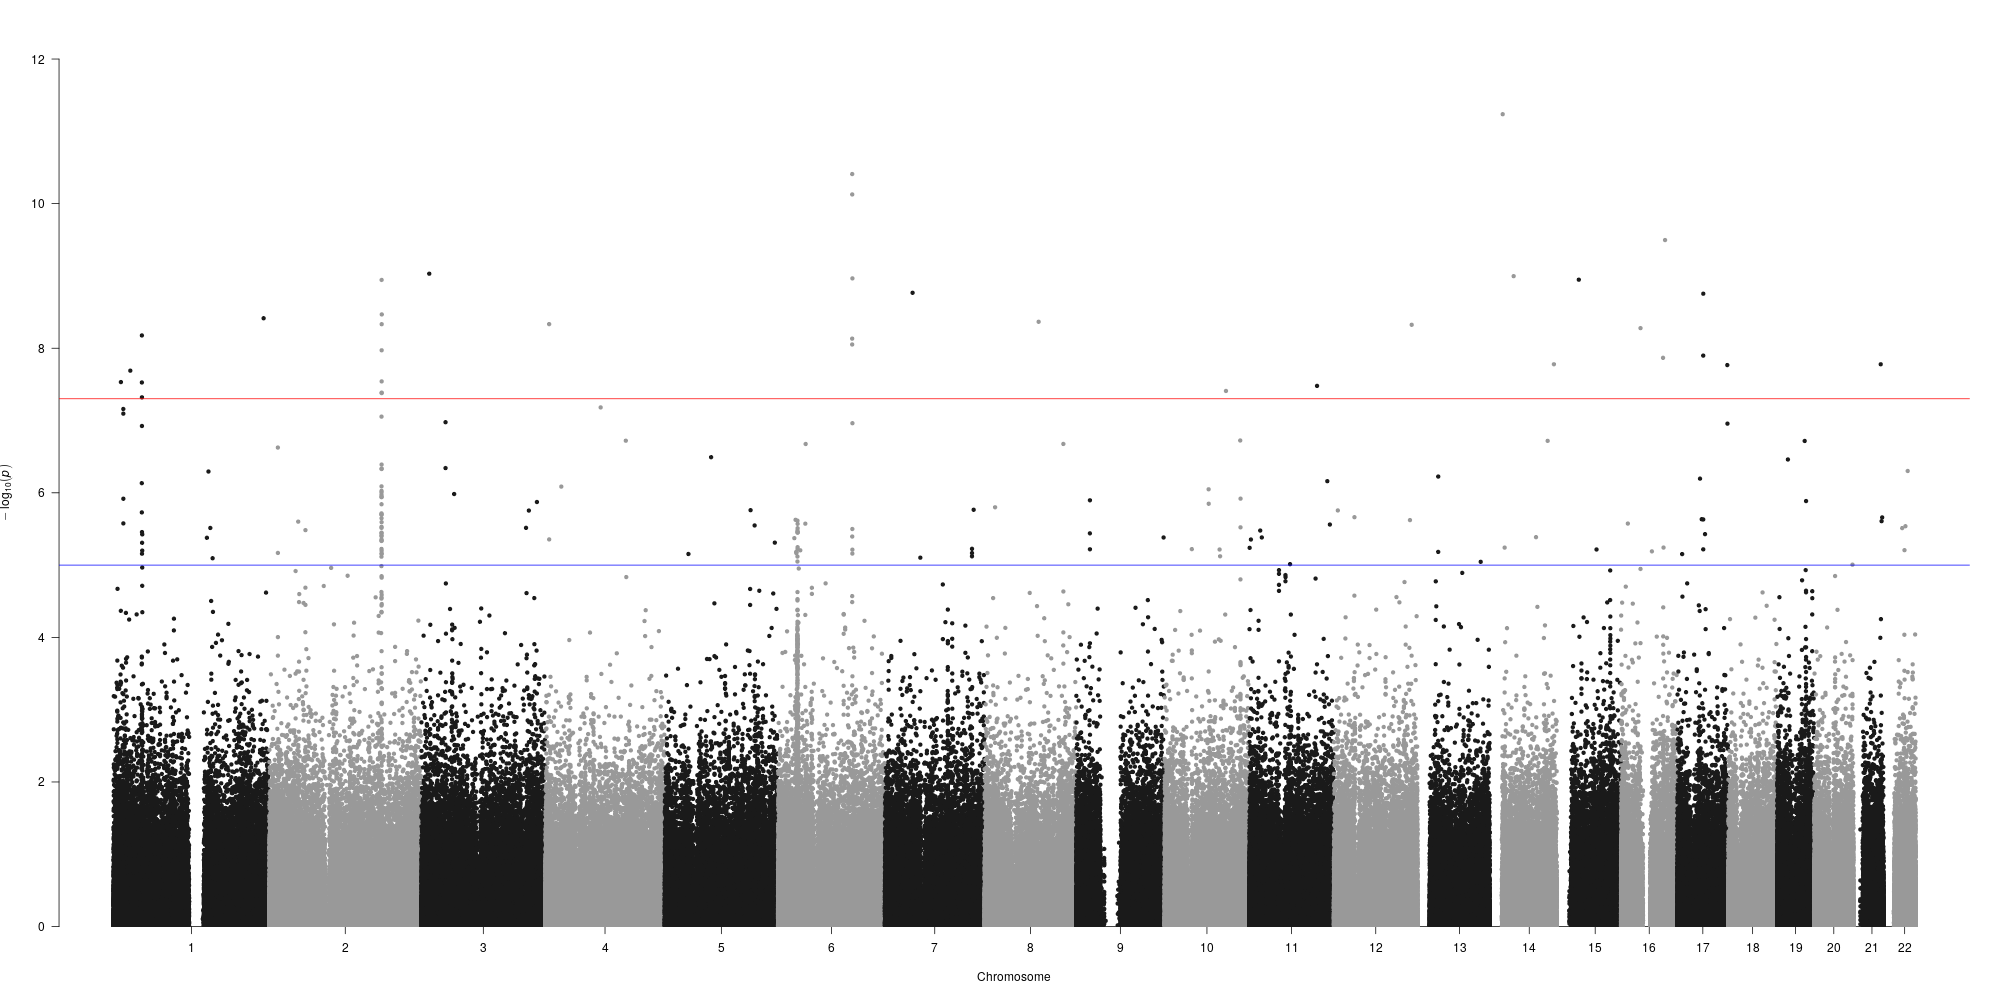
\includegraphics[width=0.8\linewidth]{figs/gwas/manhattan_LVEDV_automatic_adj.png}
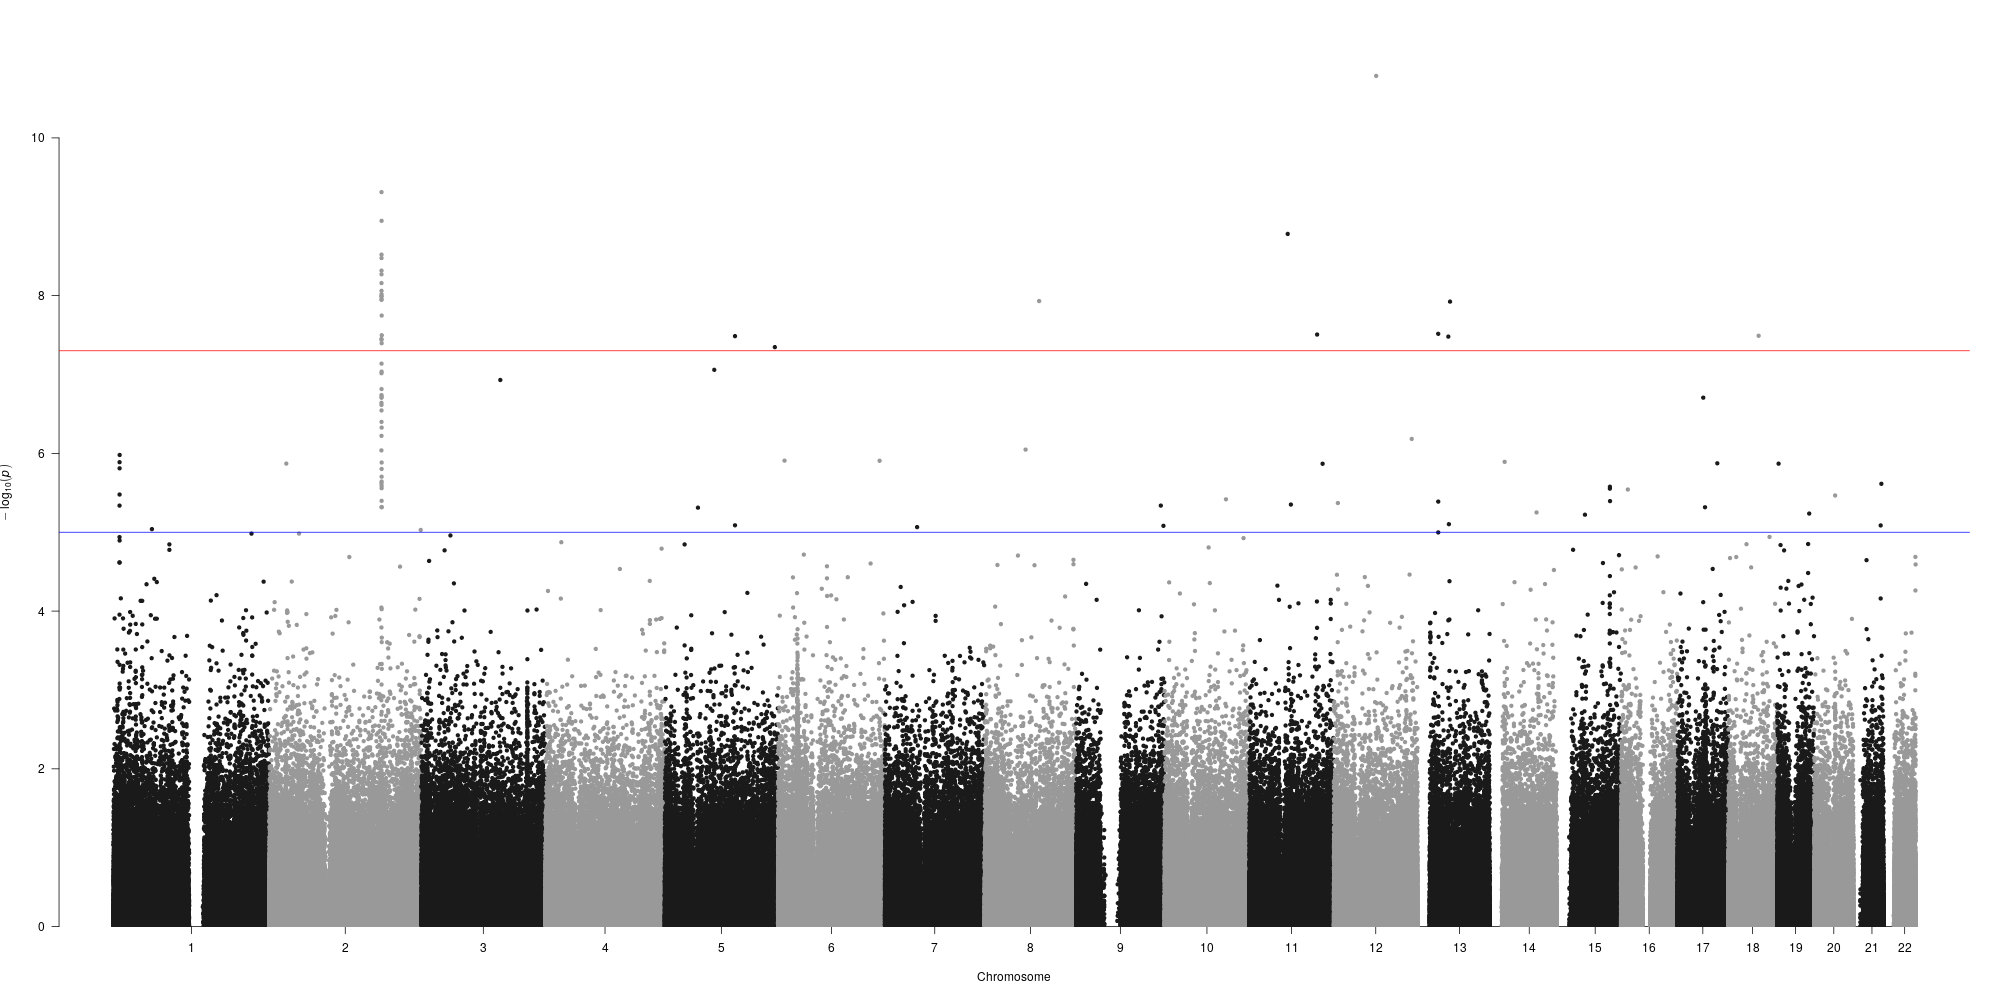
\includegraphics[width=0.8\linewidth]{figs/gwas/manhattan_LVM_automatic_adj.png}
\caption{Manhattan plots for LVEDV and LVM.}
\end{figure}


\subsection{Dimensionality reduction of 3D cardiac meshes}
Figure \ref{fig:pca_vs_coma} shows a comparison of the reconstruction error obtained through PCA and CoMA, as a function of the number of the components $K$ of the latent space. 

\begin{figure}
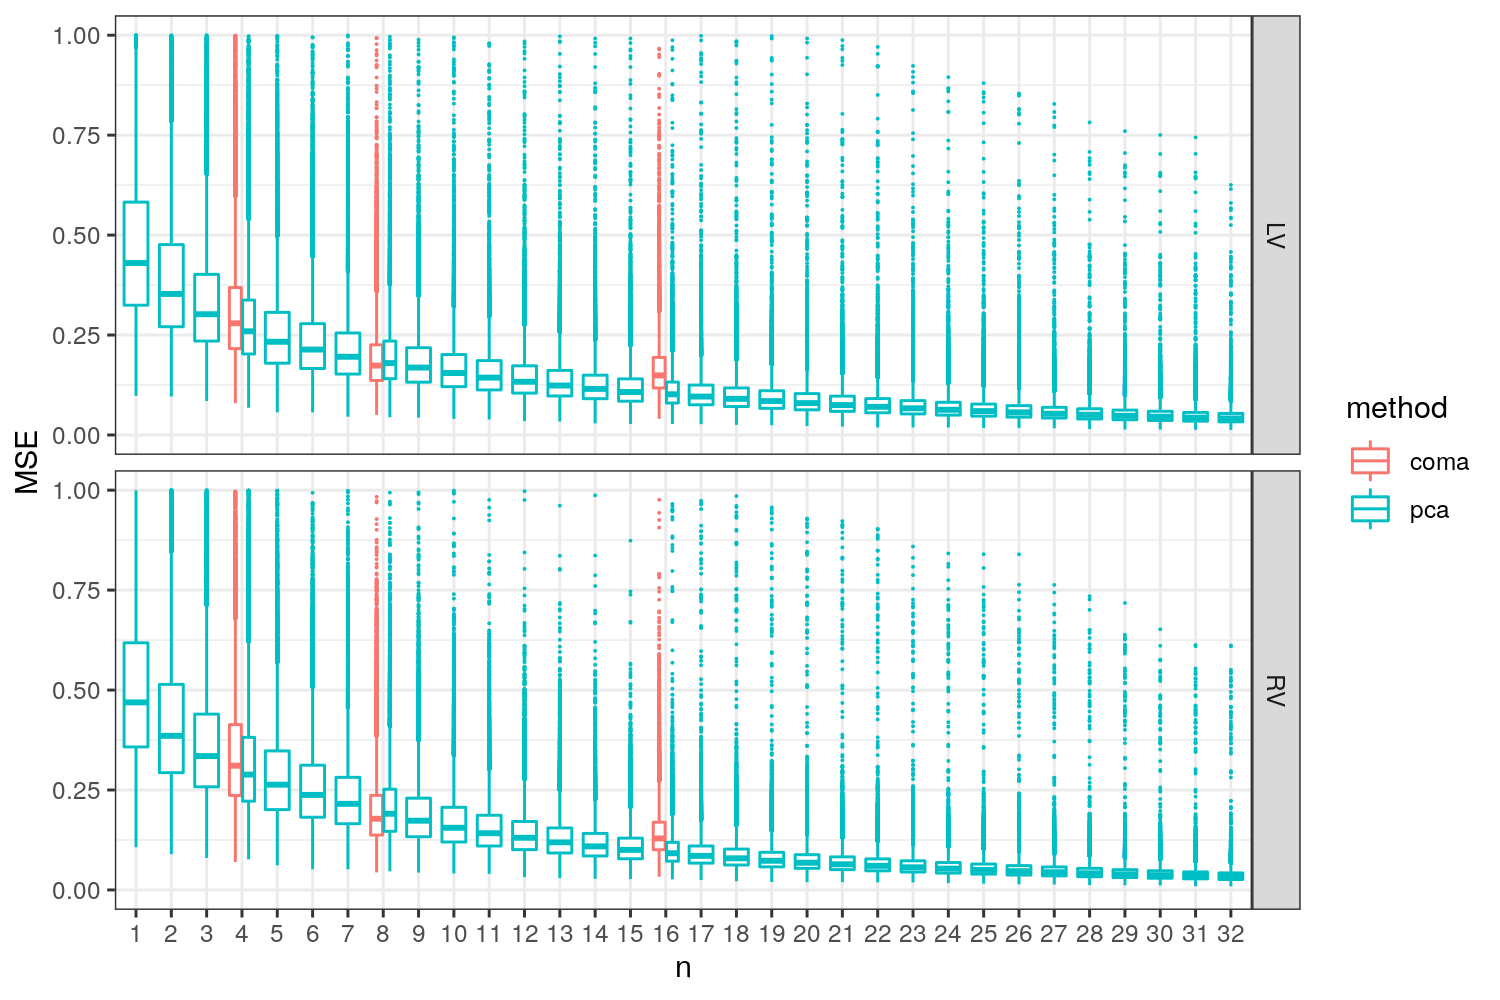
\includegraphics[width=\linewidth]{figs/mse_pca_vs_coma.png}
\caption{Dependence of the reconstruction error with the number of components in the latent space, for PCA and CoMA. \textcolor{red}{If the original and reconstructed shapes had nothing to do with each other the expected value of MSE would be around 2.}}
\label{fig:pca_vs_coma}
\end{figure}


\begin{figure}
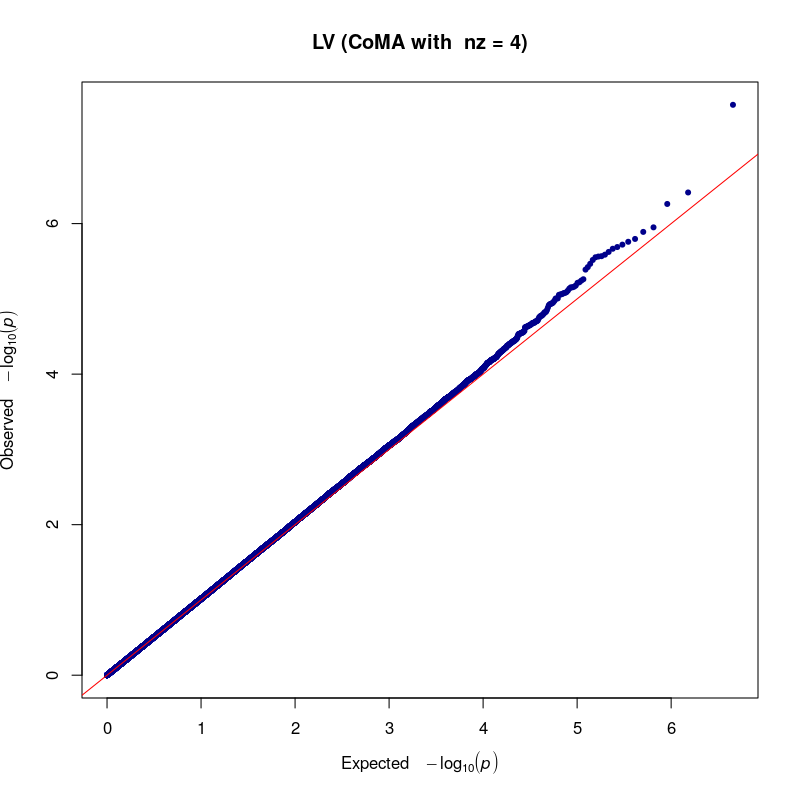
\includegraphics[width=\linewidth]{figs/gwas/2020-04-24_11_03_10_723719__LV__nz__4__gwas__qqplot__inv_norm__GBR.png}
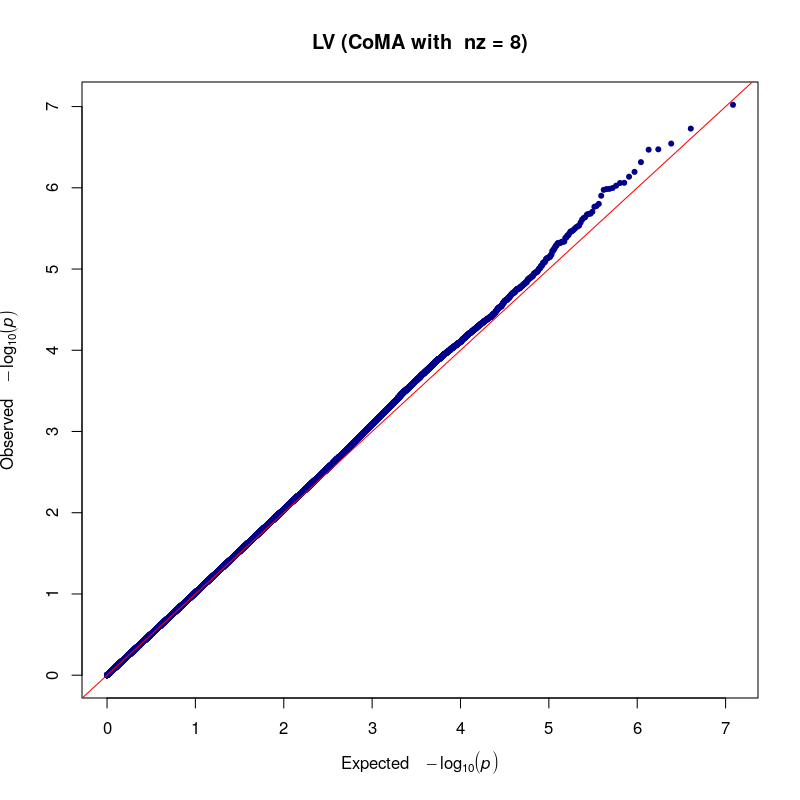
\includegraphics[width=\linewidth]{figs/gwas/2020-04-26_07_36_30_873605__LV__nz__8__gwas__qqplot__inv_norm__GBR.png}
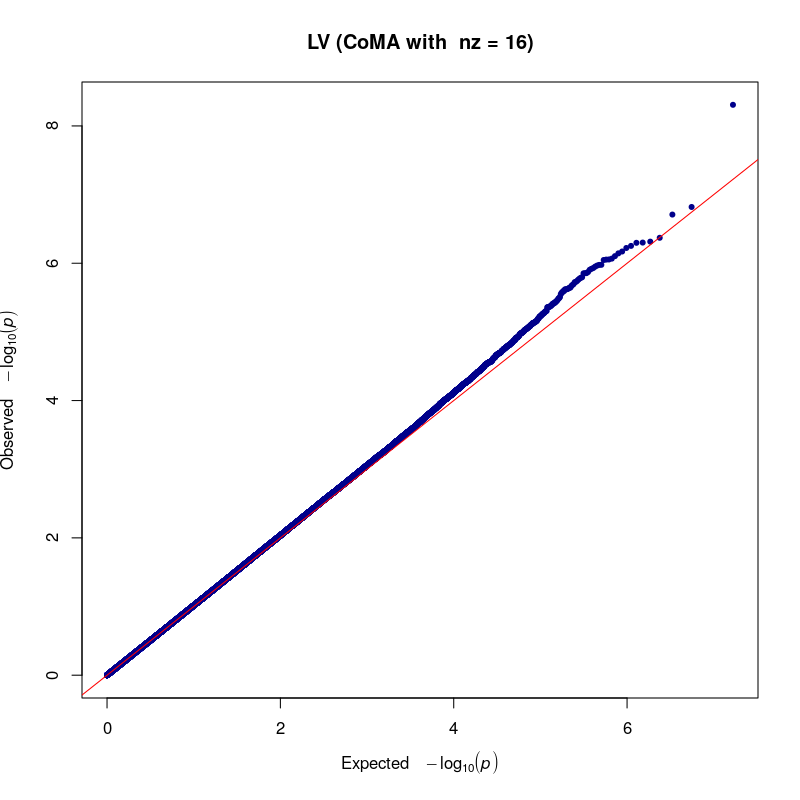
\includegraphics[width=\linewidth]{figs/gwas/2020-04-24_13_19_26_631106__LV__nz__16__gwas__qqplot__inv_norm__GBR.png}
\caption{Q-Q plot of the GWAS $p$-values for LV (the identity line corresponds to a uniform distribution of $p$-values.)}
\label{fig:qqplot_LV_pooled}
\end{figure}

\begin{figure}
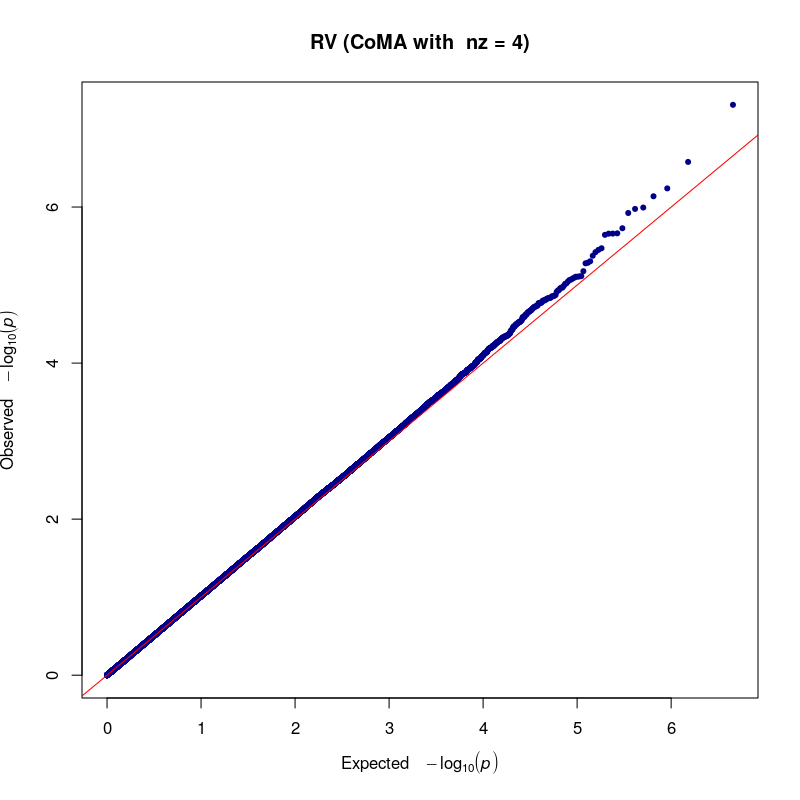
\includegraphics[width=\linewidth]{figs/gwas/2020-04-19_10_01_33_510833__RV__nz__4__gwas__qqplot__inv_norm__GBR.png}
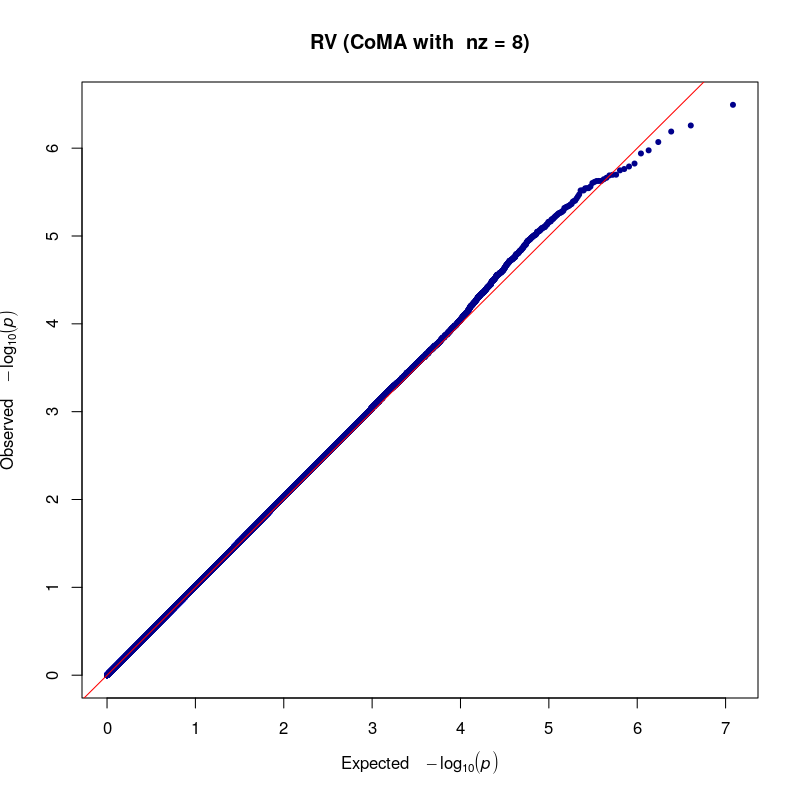
\includegraphics[width=\linewidth]{figs/gwas/2020-04-30_17_29_19_775837__RV__nz__8__gwas__qqplot__inv_norm__GBR.png}
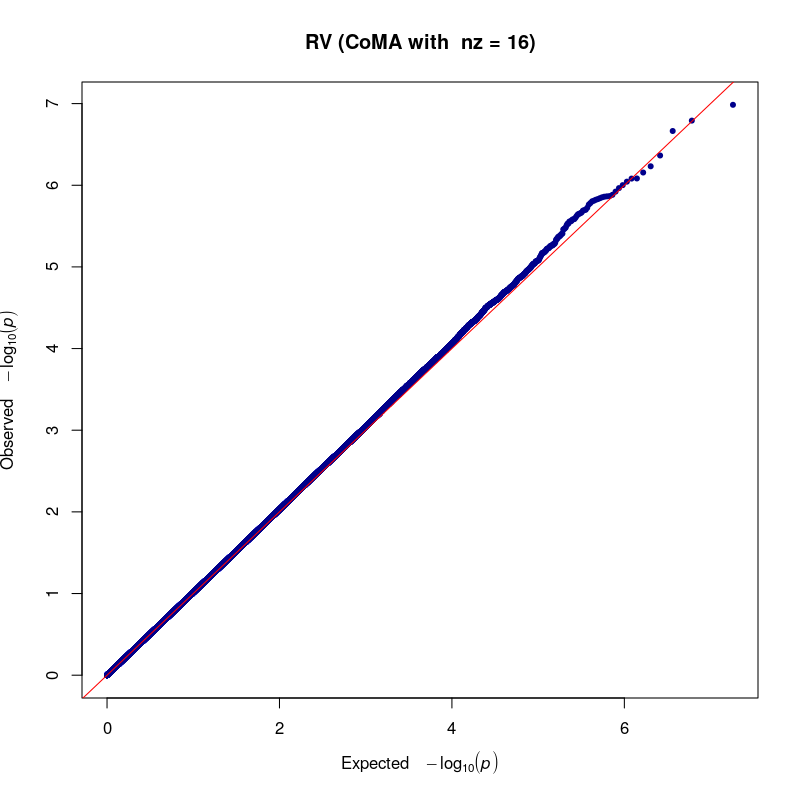
\includegraphics[width=\linewidth]{figs/gwas/2020-04-19_03_11_19_339030__RV__nz__16__gwas__qqplot__inv_norm__GBR.png}
\caption{Q-Q plot of the GWAS $p$-values for RV (the identity line corresponds to a uniform distribution of $p$-values.)}
\label{fig:qqplot_RV_pooled}
\end{figure}

\begin{figure}
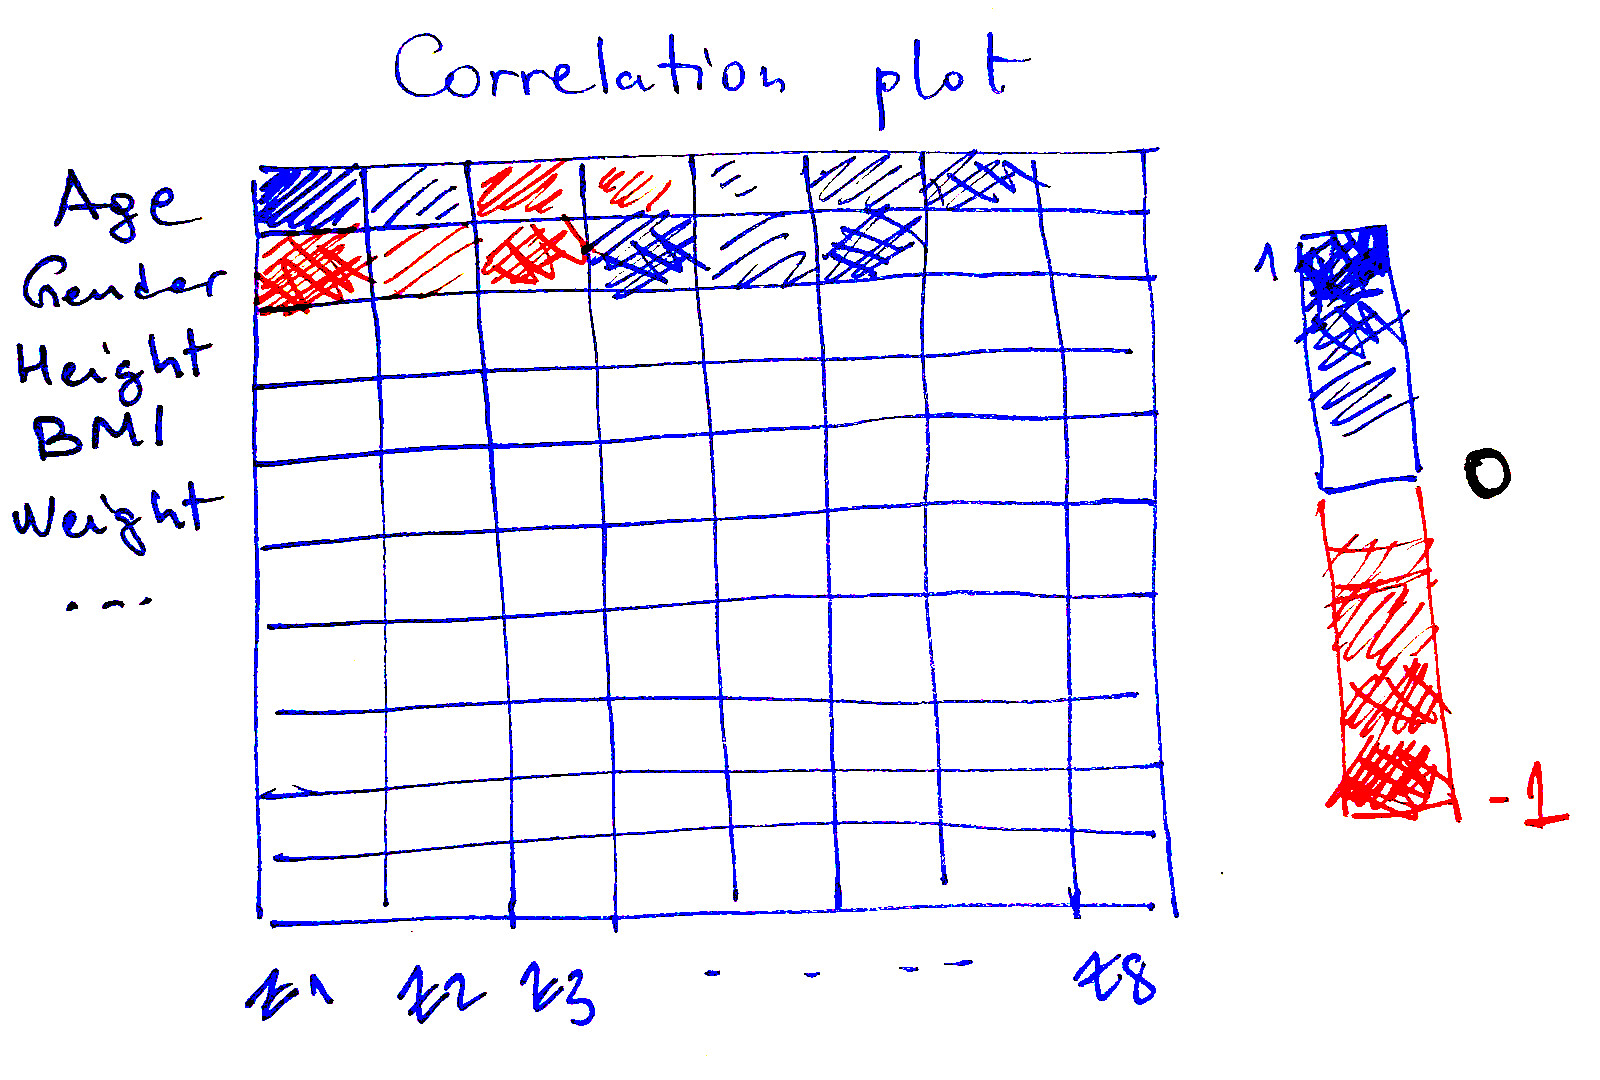
\includegraphics[width=\linewidth]{figs/corrplot_z_vs_demographic_data.jpeg}
\caption{Correlation plot of the components of the latent space against demographic data.}
\end{figure}


\subsection{Morphological interpretation of the latent basis}

\begin{center}
\begin{tabular}{ |c|c|c|c| } 
\hline
Feature & Interpretation & \# of GWAS hits \\
\hline
$z_1^{\text{LV}}$ & sphericity & 3 \\ 
\hline
$z_2^{\text{LV}}$ & orientation of mitral valve & 2\\ 
\hline
$z_3^{\text{LV}}$ & thickening of miocardium & 1 \\ 
\hline
$z_1^{\text{RV}}$ & ??? & 2 \\ 
\hline
$z_2^{\text{RV}}$ & ??? & 2 \\ 
\hline
$z_3^{\text{RV}}$ & ??? & 1 \\ 
\hline
$z_1^{\text{LA}}$ & ???  & 1 \\ 
\hline
$z_2^{\text{LA}}$ & ??? & 0 \\ 
\hline
$z_3^{\text{LA}}$ & ??? & 0 \\ 
\hline
$z_1^{\text{RA}}$ & ??? & 1 \\ 
\hline
$z_2^{\text{RA}}$ & ??? & 1 \\ 
\hline
$z_3^{\text{RA}}$ & ??? & 0 \\ 
\hline
\end{tabular}
\end{center}

\begin{figure}
\caption{color maps showing the projection along the normal vector of the deviation from the mean shape.}
\end{figure}


\subsection{GWAS}

The comparison of the Q-Q plots for PCA and CoMA shown in figures \ref{fig:qqplot_LV_pooled} and \ref{fig:qqplot_RV_pooled} reveal that the latter method produce more significant associations with the genotype. In other words, CoMA allows to extract phenotypes with higher heritability.

Manhattan plots of the components of the latent space with significant SNPs are shown in figure \ref{fig:manhattan_LV_z1_nz_8}. \textcolor{red}{I have included one Manhattan plot as an example, but I have not found genetic signal for any component for the executions that I have made so far.} 

\begin{figure}[ht]
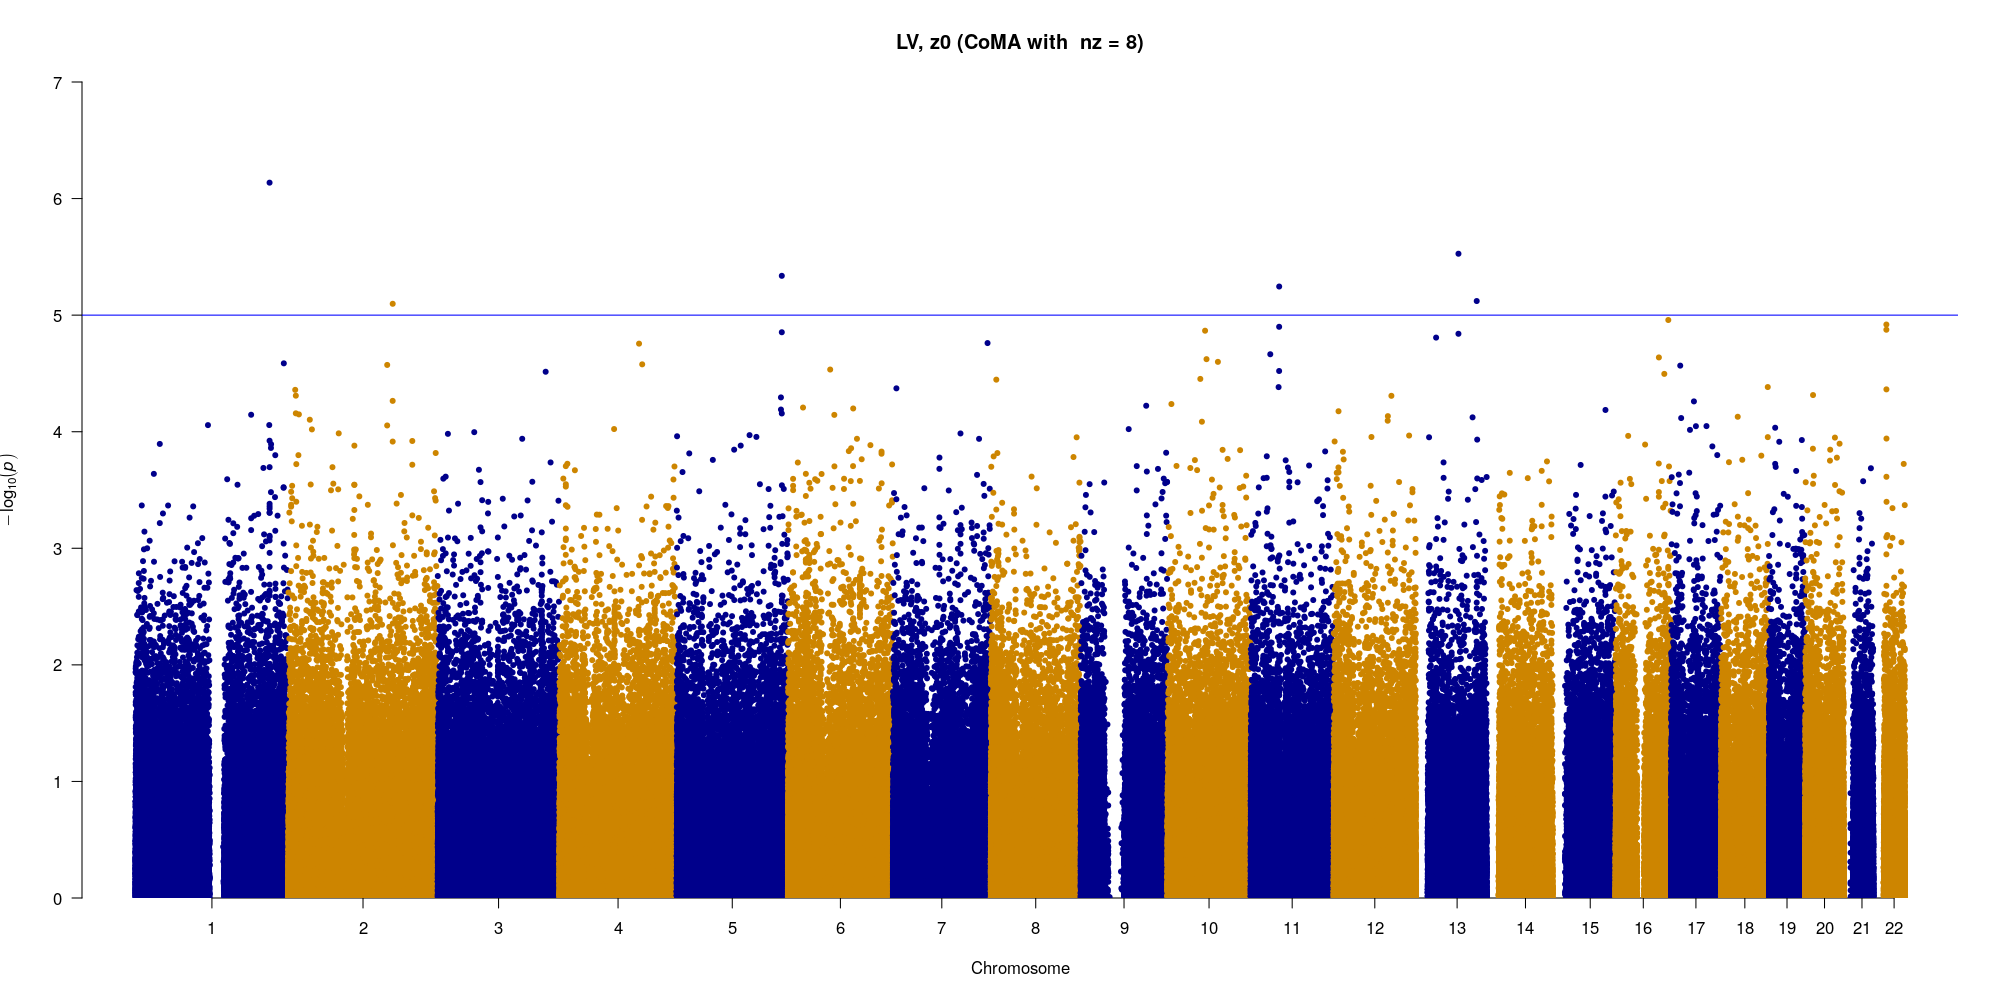
\includegraphics[width=\linewidth]{figs/gwas/2020-04-26_07_36_30_873605__LV__nz__8__gwas__manhattan__z0__inv_norm__GBR.png}
\label{fig:manhattan_LV_z1_nz_8}
\caption{Manhattan plot for one latent component of the LV.}
\end{figure}


\section{Discussion}

\textbf{Statements:}

1. \st{The convolutional mesh autoencoder learns a latent basis that allows to reconstruct the cardiac meshes with a lesser amount of components compared to PCA.} \textcolor{red}{At this stage, I was not able to obtain the results that I was expecting a priori, and my experiments show that the reconstruction error are actually similar for PCA and CoMA.}

2. The components of the latent basis have an easy visual interpretations.

3. \st{Some of the components have genetic loci associated.} \textcolor{red}{I have not found a genetic signal in the components of the latent space either.} 

The components of the latent space are significantly different for individuals with some diagnosed diseases, with respect to the healthy (or undiagnosed) individuals.

\section{Conclusions}

In this work, we have surveyed a set of indices describing structure of the different cardiac chambers in the context of genetic association analysis. In addition to commonly used clinical indices (such as chamber volume, ejection fraction and stroke volume), indices that describing the shape of the chambers were derived using two different dimensionality reduction techniques on the scaled 3D meshes: principal component analysis (PCA) and convolutional mesh-autoencoders (CoMA).

Since these latent features were learnt in a unsupervised manner, the interpretation of the latent space had to be performed \emph{a posteriori}. Some of the features were related to sphericity, wall thickness and valve orientation, whereas others had no easy interpretation.

\st{The analysis of the GWAS results yielded $\NGWASHITS$ significant genetic loci at a Bonferroni threshold of $0.05/(\NIMP\times8)$. Moreover, the significance of the associations for CoMA was higher than for PCA, confirming the suitability of that technique to extract heritable phenotypes.}

One possible future direction of this work is to consider spatio-temporal patterns by using all the phases of the cardiac cycle.

\newpage

% ---- Bibliography ----
% BibTeX users should specify bibliography style 'splncs04'.
% References will then be sorted and formatted in the correct style.
%
% \bibliographystyle{splncs04}
% \bibliography{biblio}
%

\begin{thebibliography}{8}
\bibitem{ref_rahman}
% Rahman Attar, Marco Pereaez, Ali Gooya, Xènia Albà, Le Zhang, Milton Hoz de Vila, Aaron M Lee, Nay Aung, Elena Lukaschuk, Mihir M Sanghvi, Kenneth Fung, Jose Miguel Paiva, Stefan K Piechnik, Stefan Neubauer, Steffen E Petersen, Alejandro F Frangi. \textit{Quantitative CMR population imaging on 20,000 subjects of the UK Biobank imaging study: LV/RV quantification pipeline and its evaluation}. Medical Image Analysis. Volume 56, August 2019, Pages 26-42.
Attar R, Perea\~nez M, Gooya A, Alb\`a X, Zhang L, Hoz de Vila M, Lee AM, Aung N, Lukaschuk E, Sanghvi MM, Fung K, Paiva JM, Piechnik SK, Neubauer S, Petersen SE, Frangi AF. \textit{Quantitative CMR population imaging on 20,000 subjects of the UK Biobank imaging study: LV/RV quantification pipeline and its evaluation}. Medical Image Analysis. Volume 56, August 2019, Pages 26-42.

\bibitem{ref_biffi}
Carlo Biffi, Antonio de Marvao, Mark I Attard, Timothy J W Dawes, Nicola Whiffin, Wenjia Bai, Wenzhe Shi, Catherine Francis, Hannah Meyer, Rachel Buchan, Stuart A Cook, Daniel Rueckert, Declan P O’Regan. \textit{Three-dimensional cardiovascular imaging-genetics: a mass univariate framework}. Bioinformatics, Volume 34, Issue 1, 01 January 2018, Pages 97–103.


\bibitem{ref_nayaung}
Aung N, Vargas JD, Yang CJ, Cabrera CP, Warren HR, Fung K, Tzanis E, Barnes MR, Rotter JI, Taylor KD, Manichaikul AW, Lima JAC, Bluemke DA, Piechnik SK, Neubauer S, Munroe PB, Petersen SE
\textit{Genome-Wide Analysis of Left Ventricular Image-Derived Phenotypes Identifies Fourteen Loci Associated With Cardiac Morphogenesis and Heart Failure Development}. Circulation. Vol 140, Issue 16 (2019).


\bibitem{ref_ukbb}
Bycroft C., Freeman C., Petkova D., Band G., Elliott LT., Sharp K., Motyer A., Vukcevic D., Delaneau O., O’Connell J., Cortes A., Welsh S., Young A., Effingham M., McVean G., Leslie S., Allen N., Donnelly P., Marchini J. \textit{The UK Biobank resource with deep phenotyping and genomic data}. Nature 562, 203–209 (2018). https://doi.org/10.1038/s41586-018-0579-z


\bibitem{ref_ukbb_genetics}
Bycroft C, Freeman C, Petkova D, Band G, Elliott LT, Sharp K, Motyer A, Vukcevic D, Delaneau O, Connell J, Cortes A, Welsh S, McVean G, Leslie S, Donnelly P, Marchini J
\textit{Genome-wide genetic data on ~500,000 UK Biobank participants}. bioRxiv (2017).

\bibitem{ref_spectral_graph_conv}
Defferrard M, Bresson X, Vandergheynst P. \textit{Convolutional Neural Networks on Graphs with Fast Localized Spectral Filtering.} Advances in Neural Information Processing Systems 29 (2016). 


\bibitem{ref_ukbb_cmr}
Petersen SE, Matthews PM, Bamberg F, Bluemke DA, Francis JM, Friedrich MG,Leeson  P,  Nagel  E,  Plein  S,  Rademakers  FE,  Young  AA.  Imaging  in  populationscience: cardiovascular magnetic resonance in 100,000 participants of UK Biobank-rationale, challenges and approaches. J Cardiovasc Magn Reson. 2013 Dec;15(1):46.


\bibitem{ref_multix}
Hoz de Vila M, Attar R, Perea\~nez M, Frangi AF. \textit{MULTI-X, a State-of-the-Art Cloud-Based Ecosystem for Biomedical Research}. 1726-1733 (2018). 10.1109/BIBM.2018.8621317.

\bibitem{ref_coma}
Ranjan A, Bolkart T, Sanyal S, Black MJ. \textit{Generating 3D Faces Using Convolutional Mesh Autoencoders}. ECCV 2018.

\bibitem{ref_gwas_review}
Visscher PM, Wray NR, Zhang Q, Sklar P, McCarthy MI, Brown MA, Yang J. \textit{10 Years of GWAS Discovery: Biology, Function, and Translation.} AJHG. Volume 101, Issue 1, 5-22 (2017)

\bibitem{ref_quadric_error}
Garland M, Heckbert P (1997). Surface Simplification Using Quadric Error Metrics. Proceedings of the ACM SIGGRAPH Conference on Computer Graphics (1997)

\end{thebibliography}
\end{document}
